\documentclass[12pt]{ctexart}
\usepackage[T1]{fontenc}
%\usepackage{fontspec}
%\newfontface\EmojiFont[Renderer=HarfBuzz]{Twemoji Mozilla}
\setmainfont{Times New Roman}
\usepackage[table]{xcolor}
\usepackage{graphicx,caption,subcaption} %插入多图时用子图显示的宏包
\usepackage[colorlinks=true]{hyperref} %超链接,支持unicode字符
\hypersetup{
    colorlinks,
    linkcolor={red!50!black},
    citecolor={blue!50!black},
    urlcolor={blue!80!black}
}
\usepackage{mdframed} %frame
\mdfdefinestyle{mdfexample}{
    innertopmargin=5pt,
    innerleftmargin=1cm,
    innerrightmargin=1cm,
    roundcorner=30pt,
    linecolor=green!20,
    linewidth=2pt,
    backgroundcolor=gray!20,
    frametitlerule=true,
    frametitlebackgroundcolor=grey!40!white
}
\usepackage{listings}
\usepackage[normalem]{ulem}
\usepackage{multirow,multicol,booktabs,longtable}
\usepackage{geometry}
\usepackage{siunitx}
\usepackage{colortbl}
\usepackage{blindtext}%generate dummy text
\usepackage{zhlipsum} %生成测试文本
\usepackage{array}
\usepackage{makecell}
\usepackage{tikz}
\usetikzlibrary{shapes, arrows}
\usepackage{rotating}
\usepackage{comment}
\usepackage{amsmath,amsthm}
\newtheorem{theorem}{Theorem}
% lower the symbol and make it zero width
\renewcommand{\qedsymbol}{\raisebox{-\baselineskip}{\llap{\openbox}}}
\newcommand*{\plogo}{\fbox{$\mathcal{PL}$}} % Generic dummy publisher logo
\usepackage{indentfirst}
\setlength{\parindent}{2em} %也可在正文中非全局设置
\setlength{\parskip}{0.1em}
\renewcommand{\baselinestretch}{1.0}




\begin{document}
\tableofcontents
\newpage
\section{第一段}
\fangsong 

\begin{figure}
    \centering
    \begin{subfigure}[t]{0.4\textwidth}
        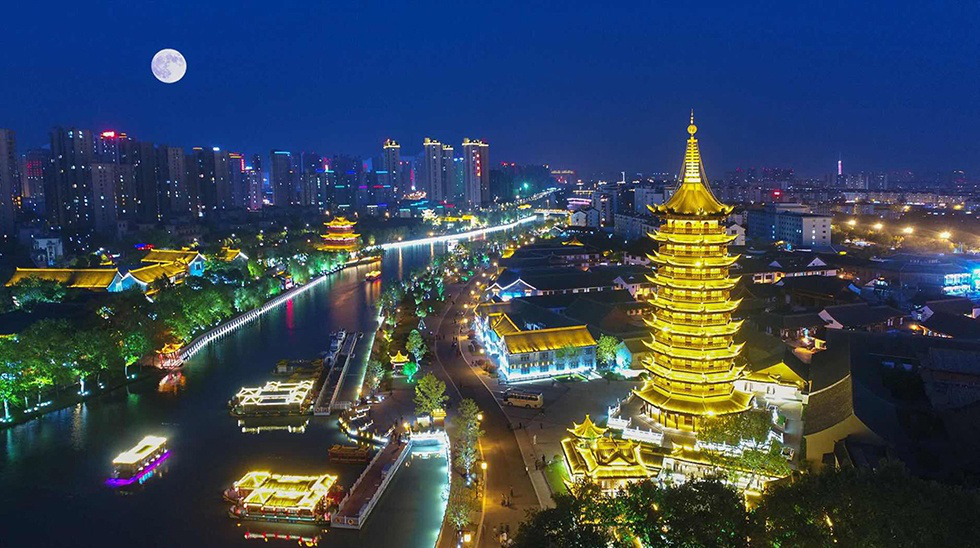
\includegraphics[width=\textwidth]{img8.png}
        \caption{First subfigure.}
        \label{fig:first}
    \end{subfigure}
    \hfill
    \begin{subfigure}[t]{0.4\textwidth}
        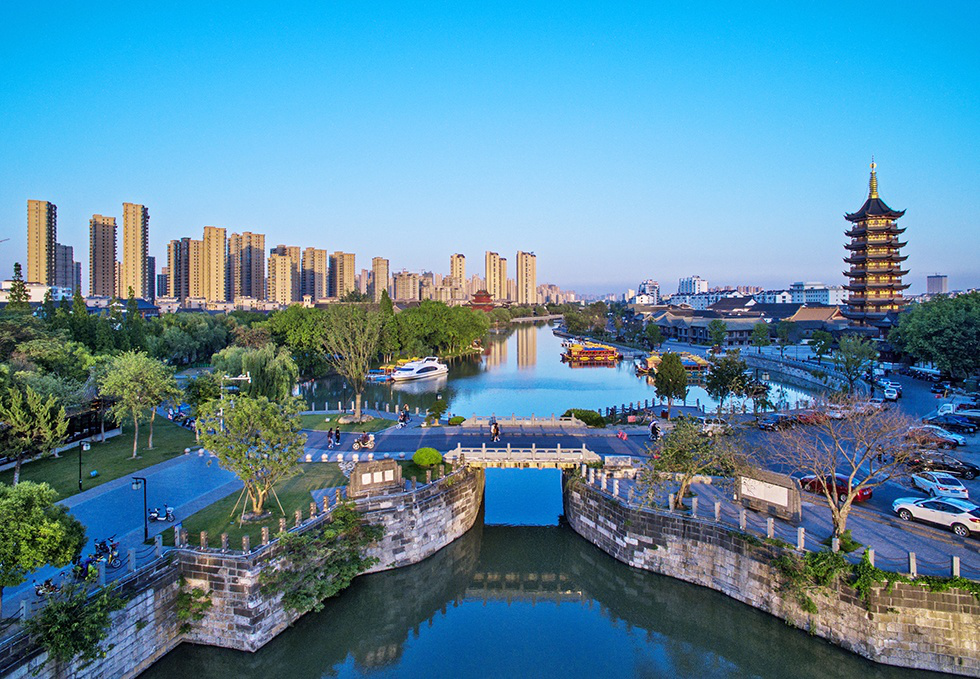
\includegraphics[width=\textwidth]{img9.png}
        \caption{Second subfigure.}
        \label{fig:second}
    \end{subfigure}
    \hfill
    \begin{subfigure}[b]{0.4\textwidth}
        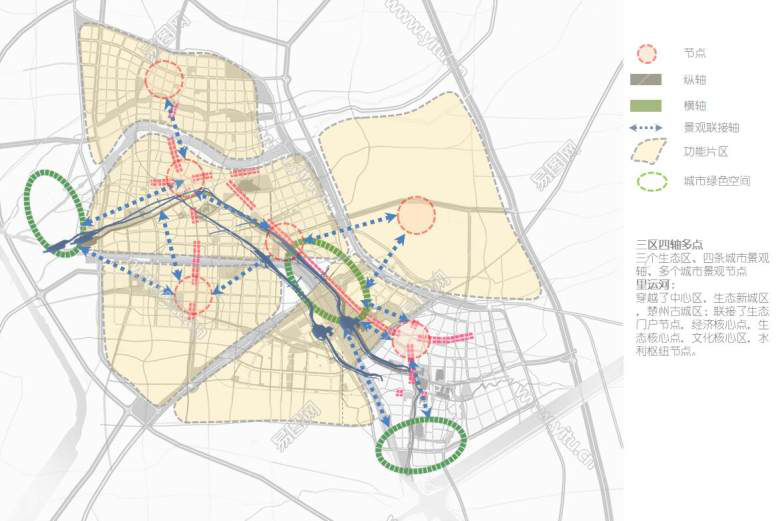
\includegraphics[width=\textwidth]{img10.png}
        \caption{Third subfigure.}
        \label{fig:third}
    \end{subfigure}
    \hfill 
    \begin{subfigure}[b]{0.4\textwidth}
        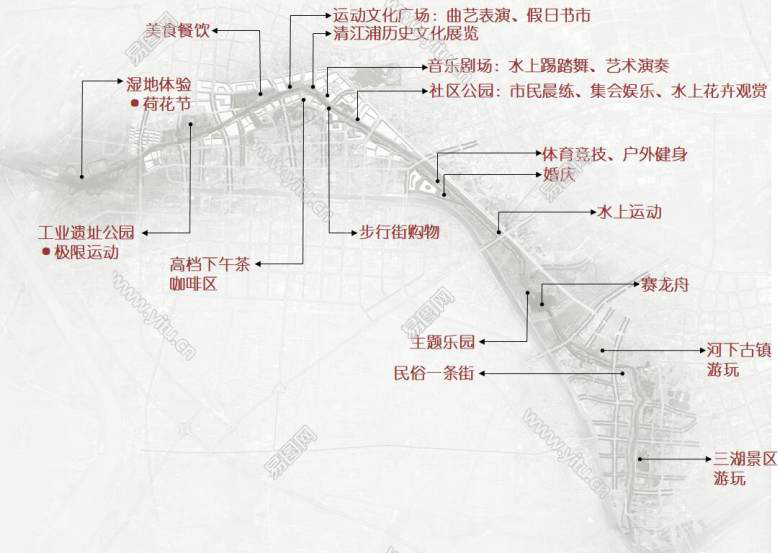
\includegraphics[width=\textwidth]{img11.png}
        \caption{Fourth subfigure}
        \label{fig:fourth}
    \end{subfigure}
            
    \caption{Vertical alignment of subfigures in \LaTeX.}
    \label{fig:figures}
\end{figure}    

你好,这是一个测试文档。\par
\rule{1pt}{\textheight} % vertical line 
\hspace{0.05\textwidth}
\parbox[b]{0.75\textwidth}{
这是新的一段。\url{http://file.finance.sina.com.cn/211.154.219.97:9494/MRGG/BOND/2020/2020-7/2020-07-13/14855437.PDF}
\vspace{0.5\textheight} % Whitespace between the title block and the publisher
		
{\indent The Publisher~~\plogo}\\[\baselineskip] % Publisher and logo
}
\begin{comment}
    \textcolor{red}{This text should NOT be displayed.}
\end{comment}
\begin{mdframed}[style=mdfexample]
    The following commands are defined for general use:\par
    \begin{enumerate}
        \item \dashuline{Hello World}
        \item \dotuline{Hello World}
        \item \emph{Hello World}
        \item \sout{Hello World}
        \item \uline{Hello World}
        \item \uuline{Hello World}
        \item \uwave{Hello World}
    \end{enumerate}
\end{mdframed}
\medskip
\zhlipsum[2-4][name=zhufu] 


\section{第二段}
\subsection{一篇文章}
病梅馆记

江宁之龙蟠,苏州之邓尉,杭州之西溪,皆产梅。
或曰:"梅以曲为美,直则无姿;以欹为美,正则无景;
以疏为美,密则无态。"固也。此文人画士,心知其意,
未可明诏大号以绳天下之梅也;
又不可以使天下之民斫直,删密,锄正,以夭梅病梅为业以求钱也。
梅之欹之疏之曲,又非蠢蠢求钱之民能以其智力为也。
有以文人画士孤癖之隐明告鬻梅者,斫其正,养其旁条,
删其密,夭其稚枝,锄其直,遏其生气,以求重价,而江浙之梅皆病。
文人画士之祸之烈至此哉!

予购三百盆,皆病者,无一完者。
既泣之三日,乃誓疗之:纵之顺之,毁其盆,悉埋于地,解其棕缚;
以五年为期,必复之全之。
予本非文人画士,甘受诟厉,辟病梅之馆以贮之。

呜呼!安得使予多暇日,又多闲田,
以广贮江宁、杭州、苏州之病梅,穷予生之光阴以疗梅也哉!
\subsection{二篇文章}
\zhlipsum[4-10][name=zhufu]
\newpage  
\subsection{乱七八糟}
\lstset{language = SQL}
% \lstset{
% numbers=left,                                        % 在左侧显示行号
% numberstyle=\tiny\color{gray},                       % 设定行号格式
% frame=none,                                          % 不显示背景边框
% backgroundcolor=\color[RGB]{245,245,244},            % 设定背景颜色
% keywordstyle=\color[RGB]{40,40,255},                 % 设定关键字颜色
% numberstyle=\footnotesize\color{darkgray},           
% stringstyle=\rmfamily\slshape\color[RGB]{128,0,0},   % 设置字符串格式
% showstringspaces=false,                              % 不显示字符串中的空格
%}
%\noindent 代码如下:
%\definecolor{dkgreen}{rgb}{0,0.6,0}
%\definecolor{gray}{rgb}{0.5,0.5,0.5}
%\definecolor{mauve}{rgb}{0.58,0,0.82}

%\lstset{
%  basicstyle=\footnotesize,       % the size of the fonts that are used for the code
%  numbers=left,                   % where to put the line-numbers
%  numberstyle=\tiny\color{gray},  % the style that is used for the line-numbers
%  numbersep=5pt,                  % how far the line-numbers are from the code
%  backgroundcolor=\color{white},  % choose the background color. You must add \usepackage{color}
%  showspaces=false,               % show spaces adding particular underscores
%  showstringspaces=false,         % underline spaces within strings
%  showtabs=false,                 % show tabs within strings adding particular underscores
%  frame=single,                   % adds a frame around the code
%  rulecolor=\color{black},        % if not set, the frame-color may be changed on line-breaks within not-black text (e.g. commens (green here))
%  tabsize=2,                      % sets default tabsize to 2 spaces
%  captionpos=b,                   % sets the caption-position to bottom
%  breaklines=true,                % sets automatic line breaking
%  breakatwhitespace=false,        % sets if automatic breaks should only happen at whitespace
%  keywordstyle=\color{blue},      % keyword style
%  stringstyle=\color{mauve},      % string literal style
%  escapeinside={\%*}{*)},         % if you want to add LaTeX within your code
%  morekeywords={*,...}            % if you want to add more keywords to the set
%}

\definecolor{codegreen}{rgb}{0,0.6,0}
\definecolor{codegray}{rgb}{0.5,0.5,0.5}
\definecolor{codepurple}{rgb}{0.58,0,0.82}
\definecolor{backcolour}{rgb}{0.95,0.95,0.92}

\lstdefinestyle{mystyle}{
    backgroundcolor=\color{backcolour},       % 设定背景颜色
    commentstyle=\color{codegreen},           % 设定注释颜色
    keywordstyle=\color{magenta},             % 设定关键词颜色
    numberstyle=\tiny\color{codegray},        % 设定行号格式
    stringstyle=\color{codepurple},           % 设定字符串格式
    basicstyle=\ttfamily\footnotesize,        % 设定代码字号
    breakatwhitespace=false,                  % sets if automatic breaks should only happen at whitespace
    breaklines=true,                          % sets automatic line breaking
    captionpos=b,                             % 设定说明位置
    keepspaces=true,                 
    numbers=left,                             % 设定行号在左边
    numbersep=5pt,                            % 设定行号与代码间距
    showspaces=false,                         
    showstringspaces=false,
    showtabs=false,                  
    tabsize=4
}

\lstset{style=mystyle}
\begin{lstlisting}
    mysql> select /* 需要查询的列 */
    from /* 需要查询的表 */
    where /* 额外的限制条件 */
    order by /* 对某一列进行排序,正序用 asc,倒序用 desc */ ;
\end{lstlisting}

这是对一个文献的引用 \cite{von2019model},我们看看效果。

\newpage 
\newgeometry{top=5mm,bottom=10mm,margin=5mm}
\begin{table*}
    \centering
    \footnotesize
    \begin{tabular}{@{}r*{10}{S[color=orange,table-format=-3.4]}@{}}
    \toprule
    & \multicolumn{3}{c}{$w = 8$} & \multicolumn{3}{c}{$w = 16$} & \multicolumn{3}{c}{$w = 32$}\\
    \cmidrule(lr){2-4} \cmidrule(lr){5-7} \cmidrule(l){8-10}
    & {$t=0$} & {$t=1$} & {$t=2$} & {$t=0$} & {$t=1$} & {$t=2$} & {$t=0$} & {$t=1$} & {$t=2$} \\
    \midrule[0.75em]  
    $dir=1$\\  
    $c$ & 0.0790 & 0.1692 & 0.2945 & 0.3670 & 0.7187 & 3.1815 & -1.0032 & -1.7104 & -21.7969\\  
    $c$ & -0.8651& 50.0476& 5.9384& -9.0714& 297.0923& 46.2143& 4.3590& 34.5809& 76.9167\\  
    $c$ & 124.2756& -50.9612& -14.2721& 128.2265& -630.5455& -381.0930& -121.0518& -137.1210& -220.2500\\  
    \addlinespace
    $dir=0$\\  
    $c$ & 0.0357& 1.2473& 0.2119& 0.3593& -0.2755& 2.1764& -1.2998& -3.8202& -1.2784\\  
    $c$ & -17.9048& -37.1111& 8.8591& -30.7381& -9.5952& -3.0000& -11.1631& -5.7108& -15.6728\\  
    $c$ & 105.5518& 232.1160& -94.7351& 100.2497& 141.2778& -259.7326& 52.5745& 10.1098& -140.2130\\  
    \bottomrule  
    \end{tabular}  
    \caption{Caption}  
\end{table*}  

\noindent
\begin{tabular}{*{3}{c}}
    \hline
    Header1 & Header 2 & Header3 \\
    \hline
    $dir=1$\\
    Column1a & Column2a & Column3a \\
    Column1b & Column2b & Column3b \\
    Column1c & Column2c & Column3c \\
    Column1d & Column2d & Column3d \\
    \hline
\end{tabular}
\quad
\begin{tabular}{@{}
    c*{3} {S[table-format = 2.2,color=orange]}
    @{}}
    \toprule
    {Header1} & {Header2} & {Header3} \\
    \midrule
    1 & 2 & 3\\
    1 & 2 & 3\\
    1 & 2 & abc\\
    \bottomrule
\end{tabular}
\noindent 
\begin{table}[h]\centering
    \begin{tabular}{@{}lcccc@{}}
    \toprule
    \multirow[c]{2}[3]{*}{Sample} & \multicolumn{2}{c}{I} & \multicolumn{2}{c}{II} \\
    \cmidrule(lr){2-3} \cmidrule(lr){4-5}
     & A & B & C & D \\
    \midrule
    S1 & \cellcolor{orange}5 & \textcolor{red}8 & 12 & 2 \\
    S2 & 6 & 9 & 2 & 6 \\
    \rowcolor{orange}
    S3 & 7 & 9 & 5 & 8 \\
    S4 & 8 & 9 & 8 & 2 \\
    \bottomrule
    \end{tabular}
\end{table}

\begin{tabular}{@{}lccccr@{}}
\toprule
{Values}
& {Values}
& {Values}
& {Values}
& {Values}
& {Values} \\
\midrule
2.3 & 2.3 & 2.3(5) & 2.3(5) & 2.3 & 2.3e8 \\
34.23 & 34.23 & 34.23(4) & 34.23(4) & 34.23 & 34.23 \\
56.78 & 56.78 & 56.78(3) & 56.78(3) & -56.78 & 56.78e3 \\
3,76 & 3,76 & 3,76(2) & 3.76(2) & +-3.76 & e6 \\
\bottomrule
\end{tabular}

\begin{table}[h]
    \label{table1}
    \caption{交易条款列举}
    \begin{tabular}{@{}r*{2}{S[color=orange,table-format=-3.4]}@{}}
        \toprule
        & 交易条款\\
        \midrule 
        立项时间 & \\
        承租人 & 丹阳水务集团有限公司\\
    \end{tabular}
\end{table}

\begin{tabular}{ll}
    Number & Text \\ \relax
    [a] & lorem ipsum \\ \relax
    [b] & lorem ipsum \\
\end{tabular}
\newpage 
\restoregeometry   
\blindtext\par
\renewcommand\arraystretch{1.3}
\noindent\begin{tabular}{
  | >{\ttfamily\raggedright\arraybackslash}p{2cm}
  | >{\sffamily\raggedright}p{2.5cm}
  | >{\sffamily}p{\dimexpr\textwidth-6\tabcolsep-4.5cm\relax} |
}
\hline
\rowcolor{gray!20}\multicolumn{1}{|l|}{\bfseries\sffamily Name} 
  & \multicolumn{1}{l|}{\bfseries\sffamily Type} 
  & \multicolumn{1}{l|}{\bfseries\sffamily Description} \\
\hline
& & \\[-2ex]
d\_super & struct disk\_superblock &
  \begin{tabular}[c]{
    | >{\ttfamily\raggedright\arraybackslash}m{1.5cm}
    | >{\sffamily\raggedright}p{1.5cm}
    | >{\sffamily}p{\dimexpr\textwidth-12\tabcolsep-5\fboxsep-7.5cm\relax} |
  }
  \firsthline
  \multicolumn{1}{|l|}{\cellcolor{gray!20}\bfseries Name} 
    & \multicolumn{1}{l|}{\cellcolor{gray!20}\bfseries Type} 
    & \multicolumn{1}{l|}{\cellcolor{gray!20}\bfseries Description} \\
  \hline
  magic & char array & magic number used to indicate if file system is generated by our OS \\
  \hline
  magic & char array & magic number used to indicate if file system is generated by our OS \\
  \hline
  \end{tabular} \\[15ex]
\hline
ibmap & void\textsuperscript{$\clubsuit$} & Pointer to l-Nodes bitmap \\
\hline
ibmap & void\textsuperscript{*} & Pointer to l-Nodes bitmap \\
\hline
ibmap & void\textsuperscript{*} & Pointer to l-Nodes bitmap \\
\hline
\end{tabular}
\begin{center}
    \begin{longtable}{|l|l|l|}
    \caption{A sample long table.} \label{tab:long} \\
    
    \hline \multicolumn{1}{|c|}{\textbf{First column}} & \multicolumn{1}{c|}{\textbf{Second column}} & \multicolumn{1}{c|}{\textbf{Third column}} \\ \hline 
    \endfirsthead

    \hline \hline
    \endlastfoot
    
    One & abcdef ghjijklmn & 123.456778 \\
    One & abcdef ghjijklmn & 123.456778 \\
    One & abcdef ghjijklmn & 123.456778 \\
    One & abcdef ghjijklmn & 123.456778 \\
    One & abcdef ghjijklmn & 123.456778 \\
    One & abcdef ghjijklmn & 123.456778 \\
    One & abcdef ghjijklmn & 123.456778 \\
    One & abcdef ghjijklmn & 123.456778 \\
    One & abcdef ghjijklmn & 123.456778 \\
    One & abcdef ghjijklmn & 123.456778 \\
    One & abcdef ghjijklmn & 123.456778 \\
    One & abcdef ghjijklmn & 123.456778 \\
    One & abcdef ghjijklmn & 123.456778 \\
    One & abcdef ghjijklmn & 123.456778 \\
    One & abcdef ghjijklmn & 123.456778 \\
    One & abcdef ghjijklmn & 123.456778 \\
    One & abcdef ghjijklmn & 123.456778 \\
    One & abcdef ghjijklmn & 123.456778 \\
    One & abcdef ghjijklmn & 123.456778 \\
    One & abcdef ghjijklmn & 123.456778 \\
    One & abcdef ghjijklmn & 123.456778 \\
    One & abcdef ghjijklmn & \\
    One & abcdef ghjijklmn & 123.456778 \\
    One & abcdef ghjijklmn & 123.456778 \\
    One & abcdef ghjijklmn & 123.456778 \\
    One & abcdef ghjijklmn & 123.456778 \\
    One & abcdef ghjijklmn & 123.456778 \\
    One & abcdef ghjijklmn & 123.456778 \\
    One & abcdef ghjijklmn & 123.456778 \\
    One & abcdef ghjijklmn & 123.456778 \\
    One & abcdef ghjijklmn & 123.456778 \\
    One & abcdef ghjijklmn & 123.456778 \\
    One & abcdef ghjijklmn & 123.456778 \\
    One & abcdef ghjijklmn & 123.456778 \\
    One & abcdef ghjijklmn & 123.456778 \\
    One & abcdef ghjijklmn & 123.456778 \\
    One & abcdef ghjijklmn & 123.456778 \\
    One & abcdef ghjijklmn & 123.456778 \\
    One & abcdef ghjijklmn & 123.456778 \\
    One & abcdef ghjijklmn & 123.456778 \\
    One & abcdef ghjijklmn & 123.456778 \\
    One & abcdef ghjijklmn & 123.456778 \\
    One & abcdef ghjijklmn & 123.456778 \\
    One & abcdef ghjijklmn & 123.456778 \\
    One & abcdef ghjijklmn & 123.456778 \\
    One & abcdef ghjijklmn & 123.456778 \\
    One & abcdef ghjijklmn & 123.456778 \\
    One & abcdef ghjijklmn & 123.456778 \\
    One & abcdef ghjijklmn & 123.456778 \\
    One & abcdef ghjijklmn & 123.456778 \\
    One & abcdef ghjijklmn & 123.456778 \\
    One & abcdef ghjijklmn & 123.456778 \\
    One & abcdef ghjijklmn & 123.456778 \\
    One & abcdef ghjijklmn & 123.456778 \\
    One & abcdef ghjijklmn & 123.456778 \\
    One & abcdef ghjijklmn & 123.456778 \\
    One & abcdef ghjijklmn & 123.456778 \\
    One & abcdef ghjijklmn & 123.456778 \\
    One & abcdef ghjijklmn & 123.456778 \\
    One & abcdef ghjijklmn & 123.456778 \\
    One & abcdef ghjijklmn & 123.456778 \\
    One & abcdef ghjijklmn & 123.456778 \\
    One & abcdef ghjijklmn & 123.456778 \\
    One & abcdef ghjijklmn & 123.456778 \\
    One & abcdef ghjijklmn & 123.456778 \\
    One & abcdef ghjijklmn & 123.456778 \\
    One & abcdef ghjijklmn & 123.456778 \\
    One & abcdef ghjijklmn & 123.456778 \\
    One & abcdef ghjijklmn & 123.456778 \\
    One & abcdef ghjijklmn & 123.456778 \\
    One & abcdef ghjijklmn & 123.456778 \\
    One & abcdef ghjijklmn & 123.456778 \\
    One & abcdef ghjijklmn & 123.456778 \\
    One & abcdef ghjijklmn & 123.456778 \\
    One & abcdef ghjijklmn & 123.456778 \\
    One & abcdef ghjijklmn & 123.456778 \\
    One & abcdef ghjijklmn & 123.456778 \\
    One & abcdef ghjijklmn & 123.456778 \\
    One & abcdef ghjijklmn & 123.456778 \\
    One & abcdef ghjijklmn & 123.456778 \\
    \end{longtable}
    \end{center}
\newpage 
\begin{turn}{90}
\tikzstyle{block} = [rectangle, draw,
    text width=10em, text centered, rounded corners, minimum height=4em]
\tikzstyle{block2} = [rectangle, draw, 
    text width=15em, text centered, fill=blue!60, minimum height=2em]
\tikzstyle{line} = [draw, -latex']
    
\begin{tikzpicture}[node distance = 2cm, auto]
    \small 
    % Place nodes
    \node[block] (cloud1) {\makecell{杭州市人民政府 \\ 认缴资金:\\ 421499.997万}};
    \node [block, right of=cloud1, xshift=2cm] (cloud2) {\makecell{浙江省开发有限责任 \\ 公司 \\ 
    认缴资金:\\ 9366.677万}};
    \node [block, right of=cloud2, xshift=2cm] (cloud3) {\makecell{杭州市拱墅区人民政府 \\ 认缴资金: 
    \\ 11400.003万}};
    \node [block, right of=cloud3, xshift=2cm] (cloud4) {\makecell{杭州市江干区人民政府 \\ 认缴资金:
    \\ 11400.003万}};
    \node [block, right of=cloud4, xshift=2cm] (cloud5) {\makecell{杭州市交通投资集团 \\ 有限公司 \\ 
    认缴资金:\\ 6333.33万}};
    \node [block, right of=cloud5, xshift=2cm] (cloud6) {\makecell{杭州市下城区人民政府 \\ 认缴资金:\\
    2850.003万}};
    \node [block2, below of=cloud3, yshift=-2cm, xshift=2cm] (cloud7) {杭州市运河综合保护开发建设集团有限责任公司};
    % Draw edges
    \path [line] (cloud1) -- node [below, xshift=0.5cm] {84.30\%}  (cloud7);
    \path [line] (cloud2) -- node [xshift=-0.8cm] {9.87\%} (cloud7);
    \path [line] (cloud3) -- node [xshift=-0.5cm] {2.26\%} (cloud7);
    \path [line] (cloud4) -- node [below] {1.71\%} (cloud7);
    \path [line] (cloud5) -- node [below] {1.23\%} (cloud7);
    \path [line] (cloud6) -- node [below] {0.57\%} (cloud7);
\end{tikzpicture}
\end{turn}
\newpage 
\bibliographystyle{unsrt}
\bibliography{ref}
\end{document}